% 旋转模型（正方形内点）：正方形 ABCD，内点 P
% 把 △BPC 绕 B 顺时针旋转 90° → △BP'A（C→A，P→P'）
% PP' 为等腰直角三角形 △BPP' 的斜边
\documentclass[tikz,border=4pt]{standalone}
\usetikzlibrary{calc, arrows.meta}
\begin{document}
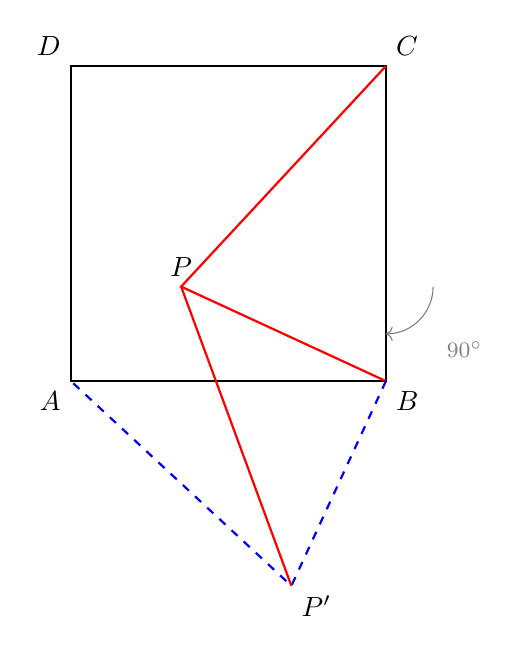
\begin{tikzpicture}[scale=1.0, thick]
  \coordinate (A) at (0, 0);
  \coordinate (B) at (4, 0);
  \coordinate (C) at (4, 4);
  \coordinate (D) at (0, 4);
  % P 在正方形内偏左下
  \coordinate (P) at (1.4, 1.2);

  % 绕 B 顺时针 90°：(x,y) → 相对 B 后 (x',y') = (y - By + Bx, -(x - Bx) + By)
  % P-B = (-2.6, 1.2)；顺时针 90°：(y, -x) = (1.2, 2.6)；P' = B + (1.2, 2.6) = (5.2, 2.6)
  % 但 P' 应落到与 C→A 对应位置（C=(4,4)→A=(0,0)），让我们重算：
  % 顺时针 90° 旋转 (x,y)→(y,-x)（绕原点）；绕 B：q-B = R·(p-B)，R(x,y)=(y,-x)
  % C-B=(0,4)→R=(4,0)→C'=B+(4,0)=(8,0)，但题意要 C→A=(0,0)。所以应是 *逆时针* 90°：R(x,y)=(-y,x)
  % C-B=(0,4)→(-4,0)→C'=(0,0)=A ✓
  % P-B=(-2.6,1.2)→(-1.2,-2.6)→P'=B+(-1.2,-2.6)=(2.8,-2.6) —— 在正方形下方外
  % 这不太理想。换成 △BPC 绕 B 逆时针旋转 90° 落到 △BP'A —— P' 在正方形外下方
  % 中考惯例：把 △BPC 绕 B 旋转使 BC 与 BA 重合（C 落到 A）—— 即逆时针 90°
  % 接受 P' 在外
  \coordinate (Pp) at (2.8, -2.6);

  % 正方形
  \draw (A) -- (B) -- (C) -- (D) -- cycle;

  % 原 △BPC（红实线）
  \draw[red, thick] (B) -- (P) -- (C);

  % 旋转后 △BP'A（蓝虚线）
  \draw[blue, dashed, thick] (B) -- (Pp) -- (A);

  % PP' 连线
  \draw[red, thick] (P) -- (Pp);

  % 旋转弧示意
  \draw[->, gray, thin] (4.6, 1.2) arc[start angle=0, end angle=-90, radius=0.6];
  \node[gray, font=\footnotesize] at (5.0, 0.4) {$90^\circ$};

  \node[below left]  at (A)  {$A$};
  \node[below right] at (B)  {$B$};
  \node[above right] at (C)  {$C$};
  \node[above left]  at (D)  {$D$};
  \node[above]       at (P)  {$P$};
  \node[below right] at (Pp) {$P'$};
\end{tikzpicture}
\end{document}
